% !TeX root = sta_paper.tex


Participants performed a visual array change detection task under four conditions formed by the cross of two presentation conditions (sequential and simultaneous) and two articulation conditions (silent and under articulatory suppression). The simultaneous presentation condition was the same as a standard visual array change detection task; in the sequential condition, however, the stimuli were presented one after another. We assume that presenting visual stimuli sequentially would afford a better opportunity to engage in strategic verbalization, if such verbalization occurs. Articulatory suppression is supposed to prevent participants from employing subvocal verbalization. The combination of simultaneous/sequential and silent/articulate conditions creates combinations of conditions that prevent participants from recruiting verbal resources (i.e. articulate, simultaneous trials) as well as those that make it more likely they could benefit from verbalization (i.e. silent, sequential trials). 


\subsection{Participants} %%%%%
Fifteen participants (8 female) between the age of 21 and 31 ({\emph M} = 25.4, {\emph SD} = 2.67) were recruited from the population of Groningen. Participants were paid \euro10 per 90-minute session and recruited through a local online social media group.

All participants were pre-screened for colorblindness and medication use that might affect their cognitive abilities, and all self-reported normal or corrected-to-normal vision and normal hearing. Furthermore, participants were only invited for subsequent sessions if they had at least 85\% correct on set-size-two trials (across all conditions) in the first session. This cut-off value was chosen based on an unpublished pilot study in which 14 out of the 15 participants performed above 85\%, and the remaining low-performing participant scored near chance (50\%) and was assumed to be ignoring the instructions. Fourteen of the participants in our final sample completed five sessions, and one participant completed four. 


\subsubsection{Apparatus and Stimuli} %%%%%
The experiment was conducted using \citet{MATLAB:2011} using the Psychophysics Toolbox extensions \citep{Brainard:1997, Kleiner:etal:2007, Pelli:1997}. The stimuli were colored squares approximately $0.65^{\circ} \times 0.65^{\circ}$ presented within a $7.3^{\circ} \times 9.8^{\circ}$ area around the screen's center. On each trial, the colors were randomly sampled without replacement from a set of nine easily-discriminable colors and presented on a gray background. The set of possible colors was identical to the one used by \citet{Rouder:etal:2008b} with the exception that black was excluded, since \citet{Morey:2011} showed that black exhibited a markedly different effect in a similar change detection task. Stimuli were shown against a neutral gray background. The items within a single array were always arranged with a minimum distance of $2^{\circ}$ from one another and participants sat approximately 50 \emph{cm} from the monitors. This setup allowed them to see the entire display without moving their heads.

Feedback was given via one of three clearly-discriminable sounds signaling a correct, incorrect, or invalid response (i.e., a key that was not assigned to either of the two valid responses). The sounds were played through headphones worn throughout the entire experiment.



\subsubsection{Procedure} %%%%%%
Within each session, participants completed one block of trials in which subvocal articulation was suppressed by requiring them to repeat aloud the syllables ``ta'' and ``da'' (\emph{articulation} block) and one block in which no such articulatory suppression was enforced (\emph{silent} block). Both the articulation and the silent blocks were further sub-divided in two blocks: one in which stimuli were presented simultaneously and one in which they were presented sequentially. The order in which blocks were completed was determined based on the participants' IDs and identical in each session. There were 504 trials in each session, yielding a total of 2,520 trials per participant (except for participant 10 who came in for four sessions, contributing 2,016 instead of 2,520 trials).

\begin{figure}[t]
 	\centering
	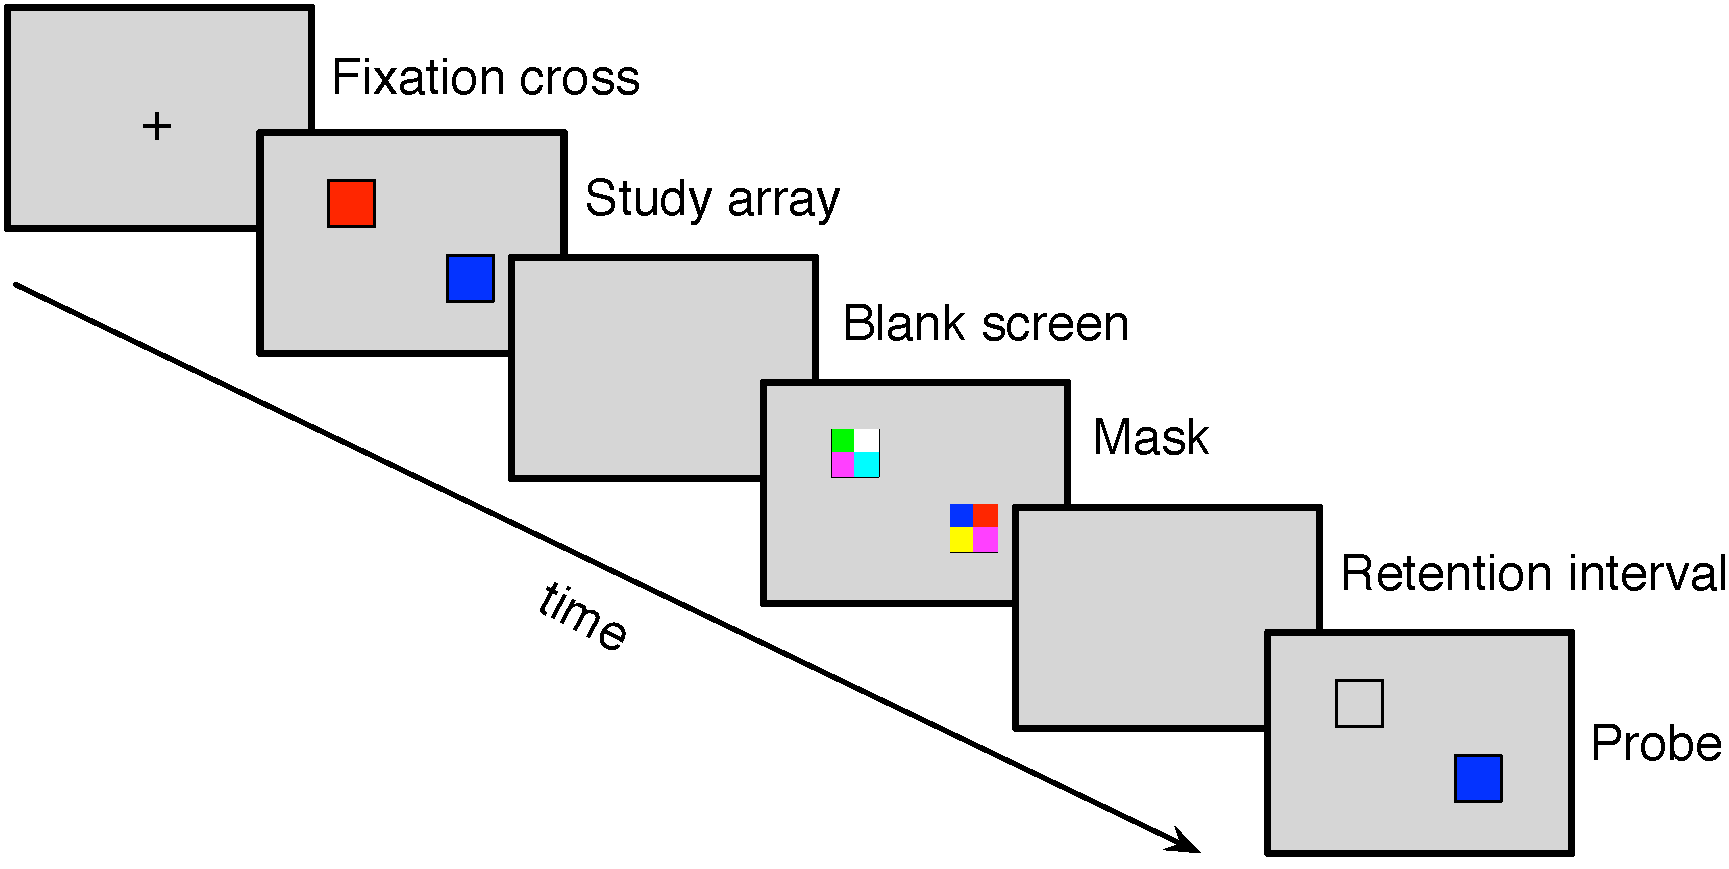
\includegraphics[width=0.5\textwidth]{figures/paradigm}
	\caption{A schematic representation of a set size two trial in the simultaneous presentation condition. For the exact timing, please consult the \emph{Procedure} sub-section. Note that the image is not to scale.}

	\label{fig:paradigm}
\end{figure}


The overall structure of the task is depicted in Figure \ref{fig:paradigm}. The trial started with a fixation cross that was on screen for 2,000 \emph{ms}. The study time in the simultaneous block was a linear function of the set size (study time = set size $\times$ 100 \emph{ms}) and the set sizes were 2, 4, and 8. In the sequential block, the stimuli appeared one after another. Each stimulus was shown with a thin, black outline and remained on the screen for 100 \emph{ms}. The stimulus color was then replaced with the background gray color and the black outline remained. After an inter-stimulus interval of 200 \emph{ms} the following stimulus appeared on screen. The outlines of all stimuli remained on screen until a mask appeared. There was a 250 \emph{ms} blank screen between the study array (or the final stimulus color in the sequential presentation) and the mask. The mask was displayed for 500 \emph{ms}. Each individual stimulus mask was made up of a $4 \times 4$ grid of colored rectangles and the colors were randomly chosen from the same color set as the whole array. After the mask disappeared, a 2,250 \emph{ms} retention interval (blank screen) delayed the onset of a single probe. The probe remained on screen until the participant made a response. Alongside the probe were thin, black outlines of the other stimuli from the study array, which were shown to prevent the participant from being unsure about which of the studied stimuli was probed.
